Para analizar la efectividad y ecuanimidad de esta nueva forma de calcular el ranking vamos a realizar una serie de test a fin de obtener un análisis cuantitativo y cualitativo
que nos permita compararlo con el clásico método de \textbf{WP}. \\
Con los test esperamos encontrar ventajas y desventajas de esta forma de medición, particularmente en escenarios donde no todos los participantes jueguen la misma cantidad de partidos.
\\

Además realizaremos una comparación de los métodos de \textbf{Eliminación Gaussiana} y \textbf{Cholesky} para ver cuál de los dos computa los rankings de manera más eficiente.
\\

En esta sección solo presentaremos los experimentos realizados y los resultados obtenidos. Las conclusiones de cada experimento
las presentaremos en la siguiente sección.

\subsection{Ranking}

Vamos a comparar la tabla de ranking obtenida a partir de un set de datos de la \textbf{ATP 2007}. Es decir calculamos el ranking a partir de la técnica \textbf{WP}, considerando
partidos ganado \/ partidos jugados, a pesar de que no todos los jugadores hayan participado de la misma cantidad de partidos. Comparándolo con el \textbf{CMM} implementado con \textbf{Cholesky}. \\


\begin{figure}[H]
    \centering
    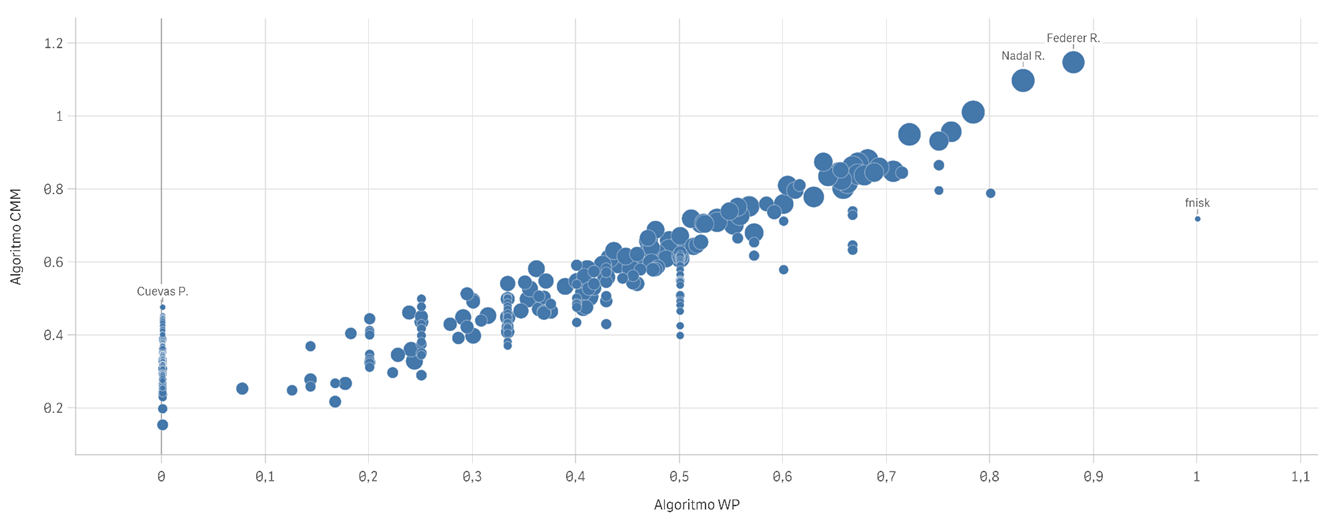
\includegraphics[width=1\textwidth]{IMG/Comparativa WP- CMM todos.png}
    \caption{Rankings para comparar WP vs CMM}
    \label{fig:Comparacion de tecnicas}
\end{figure}

\\
El grafico elegido para graficar es un gráfico de dispersión, que muestra: \\

\begin{itemize}
    \item Eje X el valor obtenido al ejecutar el algoritmo WP.
    \item Eje Y el valor obtenido al ejecutar CMM implementado con Cholesky.
    \item El tamaño de la burbuja es la cantidad de partidos jugados.
\end{itemize}


Lo que se observa en el grafico es que el ranking CMM parece darle relevancia a la cantidad de partidos jugados ya que las burbujas de los top 10 son más grandes.
Esto está dado en principio por la característica del deporte (tenis) que permite a los que ganan jugar más partidos en los torneos.
Lo que nos llamó la atención es que si observamos el Rank arrojado por WP, se observa que el primero es fnisk. El mismo es un jugador que solo jugo 1 partido y lo gano,
por lo cual tiene un 100 \% de efectividad y figura como primero. \\
Además, si observamos los top 10 del Rank WP, observamos algunas burbujas de tamaño pequeño. Esto es porque en algunos casos, este ranking beneficia jugar pocos
partidos pero ganarlos.
\\

Hemos realizado un zoom dentro del grafico para corroborar el nombre y posición de ambos rankings.
\\

\begin{figure}[H]
    \centering
    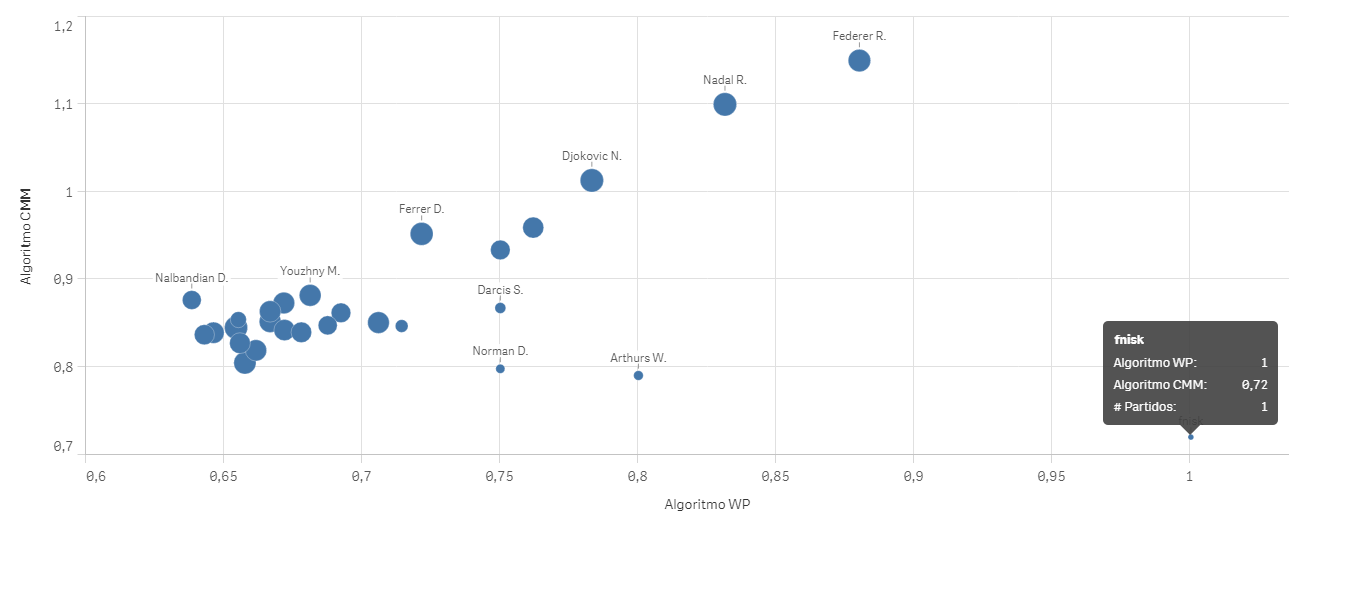
\includegraphics[width=1\textwidth]{IMG/comparativa WP - CMM zoom.png}
    \caption{Zoom de las primeras posiciones}
    \label{fig:Zoom de las primeras posiciones}
\end{figure}

\\
En el grafico se resalta el jugador fnisk y se muestra información adicional.
\\


\subsection{Justicia}

A la hora de hablar de justicia de los rankings primero debemos preguntarnos, justicia respecto a que o cual objetivo. Si observamos las pruebas para el ranking de CMM notamos ciertos movimientos de algunos equipos que no jugaban.
Estos movimientos no eran esperados por nosotros por lo que realizamos una prueba para un campeonato pequeño con el fin de replicar este problema.

Supongamos que tenemos un campeonato de 5 equipos si vemos el método de CMM, la matriz $C$ y el vector $b$ que obtendríamos en un momento inicial serian\\

\[\left C = \begin{pmatrix}
        2 & 0 & 0 & 0 & 0\\
        0 & 2 & 0 & 0 & 0\\
        0 & 0 & 2 & 0 & 0\\
        0 & 0 & 0 & 2 & 0\\
        0 & 0 & 0 & 0 & 2\\
    \end{pmatrix}\,\,
    b =
    \begin{pmatrix}
        1 \\
        1 \\
        1 \\
        1 \\
        1 \\
    \end{pmatrix}\right
\]



Donde cada posición $c_{i,j}$ representa lo que mencionamos en la sección desarrollo de cómo se construye la matriz.

Si resolvemos el sistema \textbf{(1)} con esta matriz y este vector obtendremos como vector de rankings inicial.
\begin{center}
    r =
    \begin{pmatrix}
        1/2 \\
        1/2 \\
        1/2 \\
        1/2 \\
        1/2 \\
    \end{pmatrix}
\end{center}

Si vemos el vector solución son los valores iniciales del ranking, ahora, supongamos que juega el equipo \textbf{0} y gana en el partido contra el equipo \textbf{1}, Que sucede con el ranking y los valores de cada una de las partes del sistema luego de modificarlo y buscar la solución para el ranking?

\[\left  C =
    \begin{pmatrix}
        3 & -1 & 0 & 0 & 0\\
        -1 & 3 & 0 & 0 & 0\\
        0 & 0 & 2 & 0 & 0\\
        0 & 0 & 0 & 2 & 0\\
        0 & 0 & 0 & 0 & 2\\
    \end{pmatrix}
    b =
    \begin{pmatrix}
        1,500 \\
        0,500 \\
        1 \\
        1 \\
        1 \\
    \end{pmatrix}
    r =
    \begin{pmatrix}
        1.1667 \\
        0.8333 \\
        0.5000 \\
        0.5000 \\
        0.5000 \\
    \end{pmatrix}\right
\]
Como se ve en el resultado cambian los valores de los equipos correspondientes y el ranking se modificaría haciendo que el equipo $0$ quede en primera posición y el equipo $1$ en segunda, los otros no tendrían modificaciones con lo cual hasta el momento no notamos nada que no esperábamos y no podemos replicar lo que suponemos como \'error\' visto en el gráfico.
Si repetimos los pasos pero esta vez hacemos jugar al equipo $0$ contra el $2$,para que gane el $0$, luego volvemos a calcular el ranking dándonos lo siguiente.
\newline
\[\left C =
    \begin{pmatrix}
        4 & -1 & -1 & 0 & 0\\
        -1 & 3 & 0 & 0 & 0\\
        -1 & 0 & 3 & 0 & 0\\
        0 & 0 & 0 & 2 & 0\\
        0 & 0 & 0 & 0 & 2\\
    \end{pmatrix}
    b =
    \begin{pmatrix}
        2.0000 \\
        0.5000 \\
        0.5000 \\
        1.0000 \\
        1.0000 \\
    \end{pmatrix}
    r =
    \begin{pmatrix}
        0.7000 \\
        0.4000 \\
        0.4000 \\
        0.5000 \\
        0.5000 \\
    \end{pmatrix}\right
\]

Si vemos estos resultados, notamos que no solo se modificaron los puntajes de los equipos que perdieron, si no que a su vez se modificaron los puntajes de un equipo que no jugo que en este caso es el puntaje del equipo $1$, no solo eso, si no que a su vez notamos que está manteniendo en cada una de las partidas jugadas el valor de 1/2 como promedio del ranking.
Si vemos el paper donde se detalla el método todo se deriva de cómo se construye la matriz C en \textbf{(2)}, esta misma matriz, puede ser representada como \\

\begin{center}
    $C = 2I+\displaystyle\sum_{i=1}^{total\ partidos}G_k$
\end{center}

Donde $I$, es la matriz identidad y $G_k$ tiene 0 en todas las posiciones excepto en las posiciones $G_{i,j}^k = G_{j,i}^k = -1$ y en la posiciones $G_{i,i}^k = G_{j,j}^k = 1$. Luego si a esta matriz $G$, la multiplicamos por $r$ quedándonos $r'=G_k*r$  obtendríamos que en las posiciones $i$ e $j$ nos queda $r_i-r_j$ y $r_j-r_i$ respectivamente y cero para las demás. Luego

\begin{center}
    $\displaystyle\sum_{i=1}^{N}C*r = \displaystyle\sum_{i=1}^{N}(2*I*r) = 2*\displaystyle\sum_{i=1}^{N} r_i$
\end{center}

A su vez, del otro lado del sistema, para b, podemos ver que resulta

\begin{center}
    $\displaystyle\sum_{i=1}^{N}b_i = N$
\end{center}

Finalmente si igualamos ambos resultados obtenemos

\begin{center}
    $\displaystyle\sum_{i=1}^{N}C*r = \displaystyle\sum_{i=1}^{N}b_i = N$\\
    $2*\displaystyle\sum_{i=1}^{N} r_i = N$\\
    $\implies \frac{\displaystyle\sum_{i=1}^{N} r_i}{N} = \frac{1}{2}$\\
\end{center}

Por lo que vemos que este promedio es siempre $\frac{1}{2}$ y esto explica de porque se modifican un tercero en los rankings cuando juegan dos equipos, esto no es lo que esperabamos nosotros en cuanto al metodo y tampoco parece ser muy intuitivo cuando se lo implementa. En caso de querer mas detalles sobre este metodo recomendamos leer el paper de Colley mensionado en la bibliografia.

Por otro lado, que sucede con el método de $WP$, como marcamos durante el análisis del mismo solo importa la cantidad de partidos totales y la cantidad de partidos que ganaste, pero no el resultado del partido entre otros equipos/jugadores.

Concluyendo que consideramos que los metodos parecen ser justos en cuanto al ranking que arman, en las siguientes secciones mostraremos como podremos escalar en el ranking y asi mismo como se podriamo modelar los empates y si valen la pena para definir si los metodos son justos.

\subsection{¿Importa a quien se le gana?}

En el escenario que se utiliza \textbf{WP} realmente no importa a que equipo se le gane, ya que todos los partidos tienen la misma importancia y se les asigna el mismo puntaje. Pero en el caso de \textbf{CMM} resulta más interesante plantearse esta pregunta. \\

La hipótesis que tenemos es que tomando un equipo de mitad de tabla, que denominamos \textbf{medio} el hecho de que le gane al líder de la tabla va a mejorar mucho más el ranking que derrotando al que ocupe la última posición. \\

Realizamos un test tomando al equipo \textbf{medio}, y agregando un partido victorioso contra el puntero y analizamos como se modifica su ranking. Luego tomamos la tabla inicial, es decir sin ganarle al puntero, y repetimos el experimento esta vez derrotando al último. \\

Presentamos los resultados obtenidos.

\\

\begin{table}[H]
    \caption{Posicion Inicial}
    \centering
    \begin{tabular}{c c c}
        \hline \hline
        Posición & Jugador & Ranking \\
        \hline
        1 & Federer & 1,131919 \\
        164 & Vasallo Arguello & 0,474265 \\
        334 & Vicente F. & 0,198425 \\
    \end{tabular}
\end{table}

\begin{table}[H]
    \caption{Ganandole al Primero}
    \centering
    \begin{tabular}{c c c}
        \hline \hline
        Posición & Jugador & Ranking \\
        \hline
        1 & Federer & 1,117437 \\
        141 & Vasallo Arguello & 0,508447 \\
        334 & Vicente F. & 0,198271 \\
        \hline
    \end{tabular}
\end{table}

\begin{table}[H]
    \caption{Ganandole al Ultimo}
    \centering
    \begin{tabular}{c c c}
        \hline \hline
        Posición & Jugador & Ranking \\
        \hline
        1 & Federer & 1,132469 \\
        141 & Vasallo Arguello & 0,480302 \\
        334 & Vicente F. & 0,170821 \\
        \hline
    \end{tabular}
\end{table}

\newline

Se observa una mejoría en el ranking luego de haber ganado contra el primero.
\\

\subsection{Racha ganadora}

Para estudiar la ecuanimidad del \textbf{CMM} realizamos un experimento tomando al participante del \textbf{ATP 2007} que se encontraba en el último puesto y le asignamos una racha ganadora contra los primeros diez jugadores del ranking. \\

Además este test nos permite observar como la racha de un jugador afecta al ranking global y si ganándole a los mejores realmente escala una considerable cantidad de posiciones en el ranking. \\

A continuación presentamos el ranking calculado construido de la siguiente manera: \\

\begin{itemize}
    \item Eje X el valor obtenido al ejecutar CMM implementado con Cholesky.
    \item Eje Y el valor obtenido al ejecutar CMM implementado con Eliminación Gaussiana.
    \item El tamaño de la burbuja es la cantidad de partidos jugados.
\end{itemize}

\\

\begin{figure}[H]
    \centering
    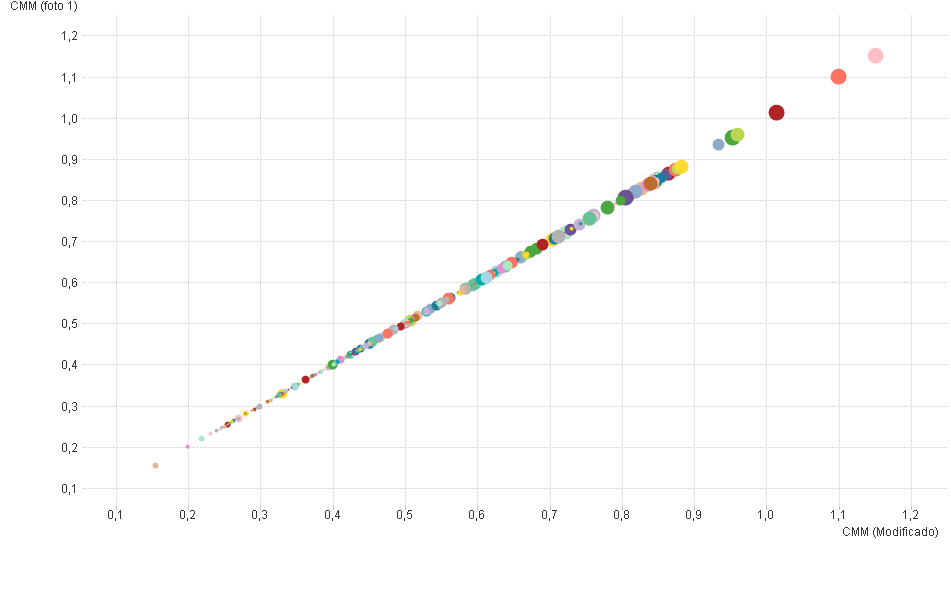
\includegraphics[width=1\textwidth]{IMG/comparativa cmm -cmm foto 0.png}
    \caption{Ranking de jugadores}
    \label{fig:Ranking de jugadores}
\end{figure}

\\
Es lógico que se observe una diagonal ya que ambos ejes son la misma métrica de CMM.
\\
Luego el experimento realizado fue agregar partidos al historial de partidos, de manera que el ultimo le gane a los 10 primeros y entender qué tipo de reacción tiene el algoritmo CMM.
\\
Para ello se realizaron 10 historiales de partidos distintos de tal forma que en cada uno de esos archivos de entrada exista un partido más que en el caso anterior y
el mismo sea una victoria del ultimo jugador del ranking vs alguno de los top 10.

\\
Para poder mostrar una evolución a medida que se van jugando los 10 partidos, hemos dejado el eje Y del gráfico con el ranking inicial, mientras que el eje X paso a ser el ranking recalculado con la agregación de partidos.\\
En el gráfico se observa mediante una flecha el salto del ranking de un partido a otro y evidencia cual es la ganancia que se tiene al ganarle a los top 10.
\\

\begin{figure}[H]
    \centering
    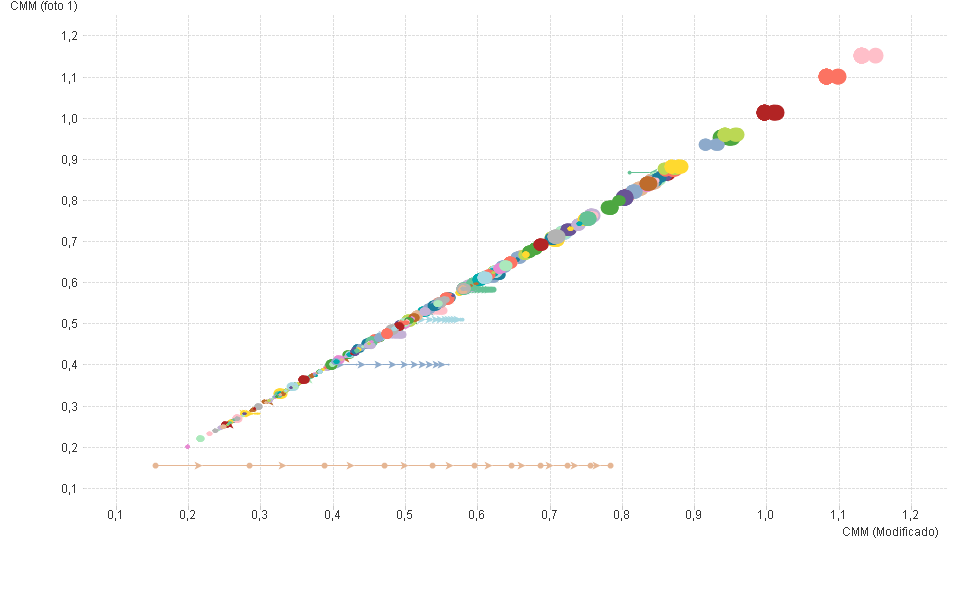
\includegraphics[width=1\textwidth]{IMG/comparativa cmm -cmm foto 10.png}
    \caption{Evolucion de jugadores con el pasar de los partidos}
    \label{fig:Evolucion de jugadores con el pasar de los partidos}
\end{figure}

\\
Por último y para entender si el jugador en la última posición podía llegar a ser primero en algún momento, hemos agregado al archivo un total de 100 partidos ganados por el ultimo contra
los top 10.
\\

\begin{figure}[H]
    \centering
    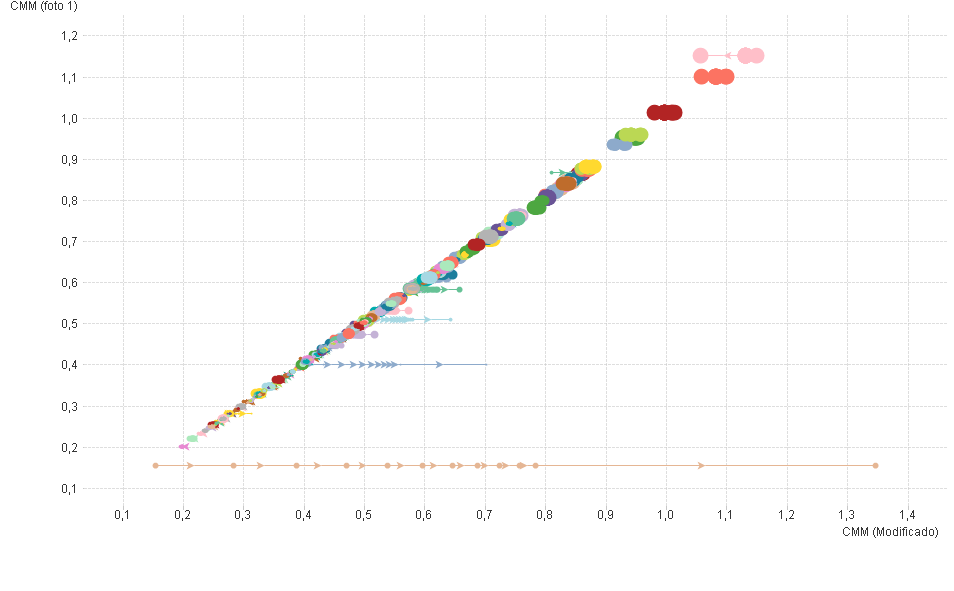
\includegraphics[width=1\textwidth]{IMG/comparativa cmm -cmm foto 100.png}
    \caption{Evolucion de jugadores con el pasar de los partidos}
    \label{fig:Evolucion de jugadores con el pasar de los partidos}
\end{figure}

\\
Y tal como vemos, si es posible pero a un costo altísimo (jugar alrededor de 100 partidos).

\\
Lo interesante es que aquellos equipos contra los que el ultimo jugador jugo también sufrieron modificaciones en su ranking. \\
A continuación se observa un zoom dentro del grafico para observar este comportamiento.
\\

El ultimo jugador del ranking se llama Verkerk M., sus partidos fueron los siguientes:

\\
\begin{table}[H]
    \caption{Partidos jugados por Verkerk}
    \centering
    \begin{tabular}{| c | c | c | c | c |}
        \hline \hline
        Nro Partido & Ganador & Sets Ganados & Perdedor & sets Perdidos \\
        \hline
        535 & de Voest R. & 2 & Verkerk M. & 0 \\
        757 & Grosjean S. & 2 & Verkerk M. & 0 \\
        832 & Hanescu V. & 2 & Verkerk M. & 0 \\
        902 & Chela J.I. & 2 & Verkerk M. & 0 \\
        1063 & Brands D. & 2 & Verkerk M. & 0 \\
        1092 & Acasuso J. & 2 & Verkerk M. & 0 \\
        1145 & Almagro N. & 2 & Verkerk M. & 0 \\
        1212 & Lapentti N. & 2 & Verkerk M. & 0 \\
        1234 & Bolelli S. & 3 & Verkerk M. & 0 \\
        \hline
    \end{tabular}
\end{table}

\\
En el siguiente grafico se observa el movimiento de ranking de los que le ganaron partidos a Verkerk, teniendo en cuenta la escalada al primer puesto de este jugador.
\\
\begin{figure}[H]
    \centering
    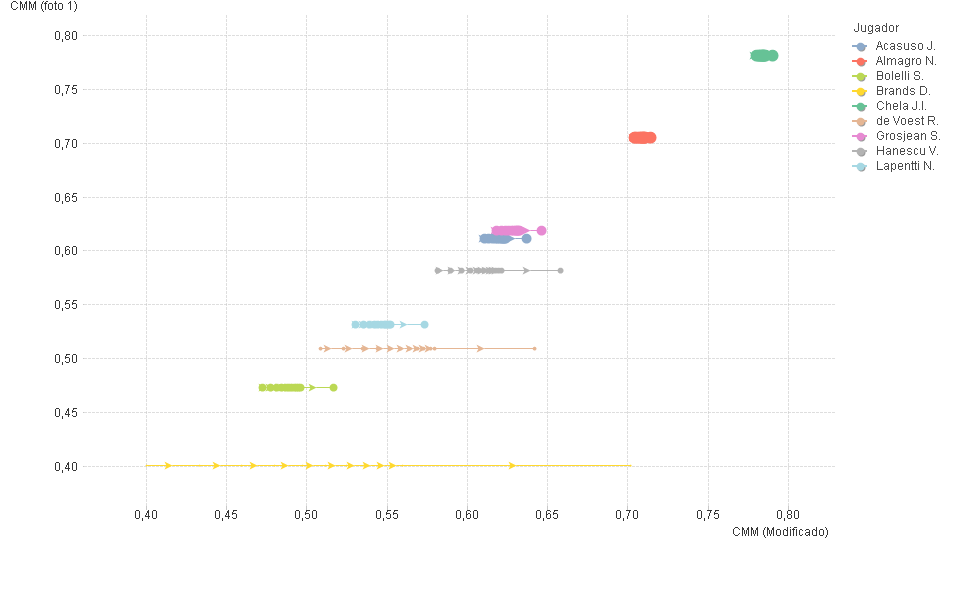
\includegraphics[width=1\textwidth]{IMG/partidos jugados vs verkerk grafico.png}
    \caption{Evolucion de aquellos que le ganaron a Verkerk}
    \label{fig:Evolucion de aquellos que le ganaron a Verkerk}
\end{figure}

\subsection{Escalando Posiciones}

Una de las consignas del trabajo era encontrar una técnica para hacer escalar en el ranking a un \textbf{equipo}, pensamos en 2 técnicas asumiendo que el torneo se encuentra en un punto donde todavía quedan partidos por jugar para saber cuántos partidos debe jugar para llegar al primer puesto y otra para variar los partidos hacia atrás viendo si es posible que llegue al primer puesto.
\\
Las primeras dos se basan en, dado un historial de partidos ya definido donde existe un jugador que esta último en el ranking, hacerlo jugar y ganar, en primer lugar con el que siempre esta primero partido a partido y en otro experimento contra el que tiene inmediatamente arriba en el ranking. Para la otra técnica se realizó un experimento tomando al jugador que este en menor posición con almenos un partido jugado e iremos variando sus partidos para tratar de ver como se modifica el ranking, por ultimo compararemos todas estas etrategias.
\\
Las siguientes estrategias fueron implementadas de manera que los algoritmos terminen la ejecución al llegar al primer puesto, arrojando la cantidad de partidos en total que debió jugar, y ganar, ese jugador para las dos primeras técnicas y para la última cuando se modificaron todos los partidos.

A continuación se muestran los análisis.

\subsubsection{Ganarle siempre al primero}

\begin{figure}[H]
    \centering
    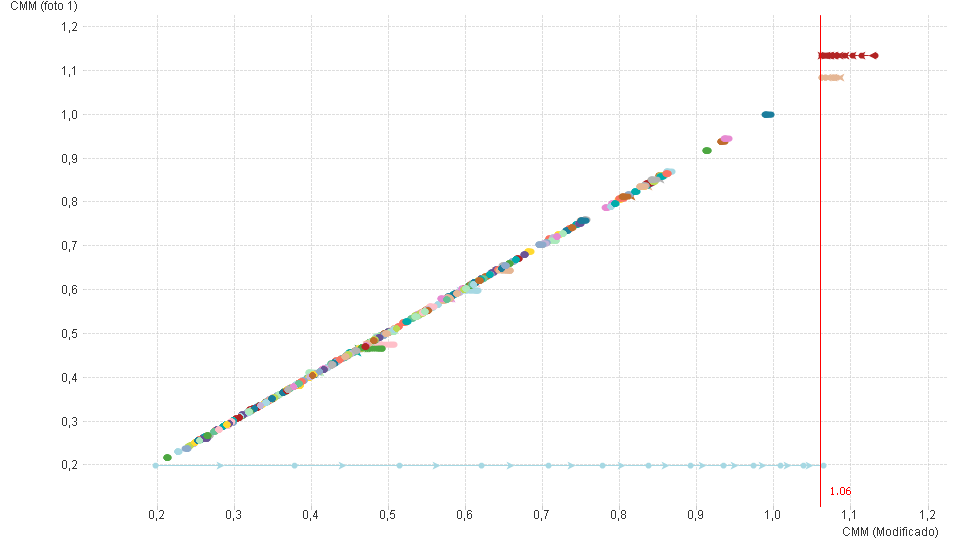
\includegraphics[width=1\textwidth]{IMG/estrategia 5.png}
    \caption{Ganarle siempre al primero}
    \label{fig: Ganarle siempre al primero}
\end{figure}

En este grafico se observa lo siguiente.\\
Cada burbuja es un jugador, el eje de las X es el Rank que arroja CMM para las distintas fechas jugadas, mientras que el eje Y tiene el Rank de CMM base para
realizar el análisis y comparar la evolución de los jugadores.

En este grafico se observa que el crecimiento es rápido en un inicio y luego va reduciendo su velocidad de crecimiento.
Se observa que el algoritmo necesita de 12 fechas para llegar a la cima del campeonato, validando nuestra teoría.\\

Se observa también una línea de referencia que indica cuando llega el jugador a superar al primero del ranking.\\

\subsubsection{Ganarle al que esta inmediatamente arriba}
\\

\begin{figure}[H]
    \centering
    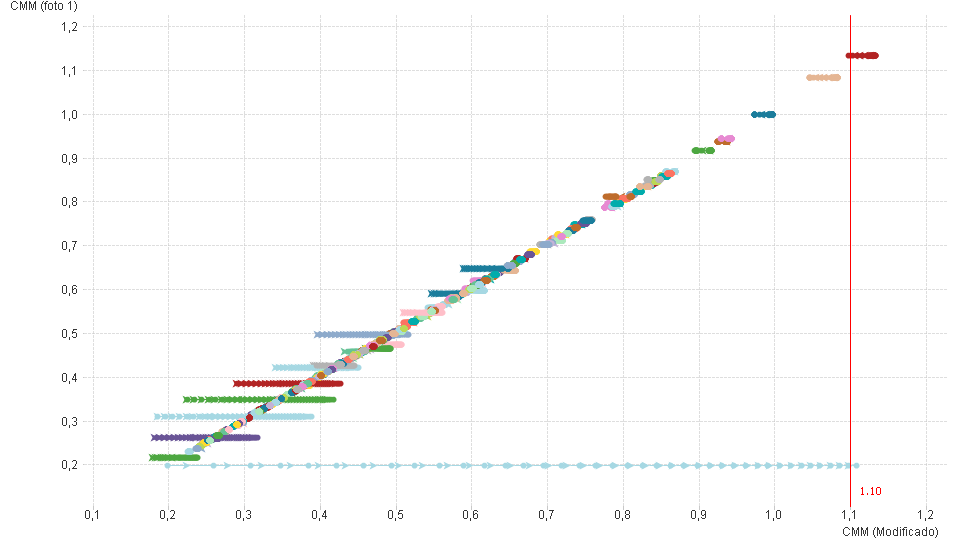
\includegraphics[width=1\textwidth]{IMG/estrategia 4.png}
    \caption{Ganarle siempre al que esta inmediatamente arriba}
    \label{fig:Ganarle siempre al que esta inmediatamente arriba}
\end{figure}

En este grafico se observa que el crecimiento es lento y que se necesitan aproximadamente 40 fechas para llegar a la cima del campeonato.\\

Se observa también una línea de referencia que indica cuando llega el jugador a superar al primero del ranking.\\

\subsubsection{Modificando los resultados}

Para esta técnica lo que se realizo fue elegir un equipo que se encuentre en la última posición e intentar hacer que suba las posiciones modificando los resultados de sus partidos perdidos.

\textbf{Porque esto es posible?}

Esto es posible porque el resultado del partido, ya sea ganado o perdido, se encuentra en el vector b, con lo cual basta con modificar ese vector para poder ejecutar otra vez el ranking.

Si bien no se utilizó en esta experimentación, podríamos utilizar la ventaja de tener una matriz factorizada para realizar solamente los algoritmos de backgward substitution y forward substitution para obtener los resultados más rápido.
De igual manera para implementar esto lo que se hizo fue ejecutar una cantidad de veces igual a la cantidad de partidos ganados del equipo elegido y terminar cuando no tenga más resultados que cambiar o cuando haya llegado a la primera posición. En cada iteración lo que se hizo fue modificar el resultado del partido contra el equipo que perdió y luego volver a calcular el ranking.
\newpage
\textbf{Porque elegimos experimentar con el ultimo?}

Debido a que con la prueba queremos ver si es posible llegar a la primera posición y  empezamos planteando que no es posible para equipos que jugaron pocos partidos.
De igual manera estos experimentos podrian realizarse para cualquiera de los equipos, siempre esperando que sucedan cualquiera de los tres escenarios que pensamos que pueden suceder. En primer lugar, si es el equipo que se encuentra primero, va a seguir primero. En segundo lugar, para el equipo que se encuentre en cualquier otra posicion pueden pasar dos cosas, que pase a la primera posicion, o que no peuda llegar nunca que es lo que vamos a ver que puede suceder.

\textbf{Los resultados fueron los esperados?}

Realmente como planteamos anteriormente esperábamos que no llegue a la primera posición, de igual manera el salto que hizo al ganar sus partidos no fue el esperado, llego a mitad de tabla como se puede ver en el siguiente gráfico.

\begin{figure}[H]
    \centering
    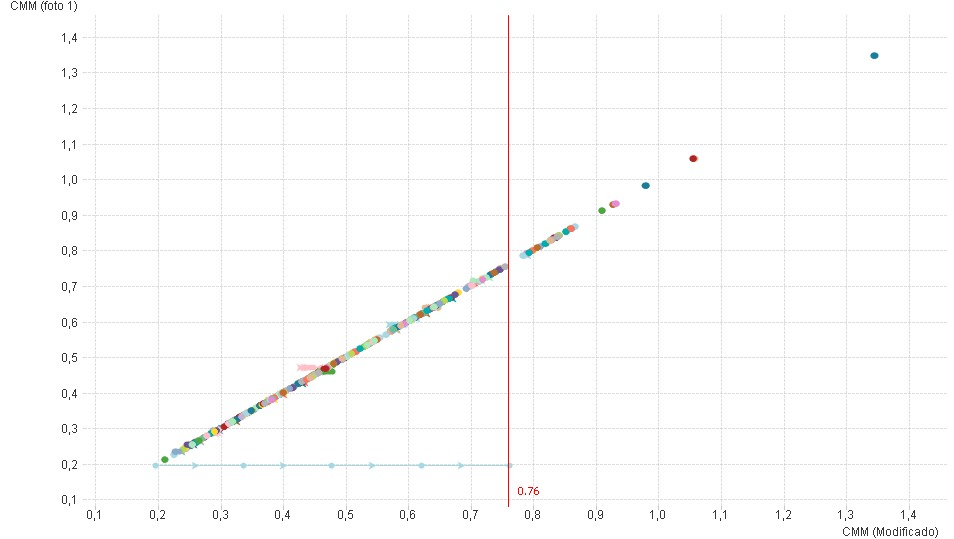
\includegraphics[width=1\textwidth]{IMG/modificandob.jpg}
    \caption{Modificando el vector b}
    \label{fig:Modificando partidos perdidos}
\end{figure}

Si analizamos el grafico anterior podemos ver que se modifican 5 partidos,estos son contra equipos que están delante del equipo seleccionado en el ranking y este llega a mitad de tabla.

\subsubsection{Comparación de Estrategias}
Si nos pusiéramos a analizar las estrategias anteriores con el fin de encontrar similitudes y diferencias, podemos notar que en cuanto a tiempos de ejecución o resolución del sistema tardarían lo mismo, debido a que como mencionaremos en el análisis cuantitativo la cantidad de partidos no afecta el tiempo de resolución del mismo.
Por otro lado, la principal diferencia entre una técnica y la otra es que si agregamos partidos a un ranking, siempre llegaríamos a una cantidad de partidos finita para terminar en primera posición, sea la cantidad que sea, diferente es en la técnica de cambiar resultados que podríamos no llegar a estar en primera posición como se ve en el ejemplo anterior, como lo pudimos ver en los gráficos anteriores.

\subsubsection{Empate}

Dado que ninguno de los metodos modela los empate, decidimos establecer que los empates sean tomados como un partido ganado para cada uno de los equipos, con el fin de ver como se verian afectados los rankings a comparacion del metodo original que no los toma.
En ambos metodos se realizaron test con un conjunto de pocos equipos y pocos partidos para ver como resultaban los rankings.
Si hacemos el siguiente historial de partidos para 6 equipos.
\begin{center}
    \begin{tabular}{| 1 | 1 | 1 | 1 |}
        \hline
        Equipo1 & goles equipo 1 & Equipo2 & goles equipo 2\\ \hline
        1 &16 &4 &13\\
        2 &38 &5 &17\\
        2 &0 &6 &1\\
        3 &34 &1 &21\\
        3 &23 &4 &10\\
        4 &31 &1 &6\\
        5 &0 &6 &1\\
        5 &38 &4 &23\\
        6 &1 &2 &0\\
        6 &1 &5 &1\\
        4 &1 &6 &1\\
        3 &1 &1 &1\\
        3 &1 &2 &1\\
        \hline
    \end{tabular}
\end{center}

Para $WP$ obtuvimos los siguientes resultados
\begin{center}
    \begin{tabular}{| 1 | 1 | 1 |}
        \hline
        Equipo & posicion Sin contar empate& posicion contando empate\\ \hline
        1&0.333333 & 0.500000 \\
        2&0.500000& 0.666667\\
        3&1.000000& 1.000000\\
        4&0.250000& 0.400000\\
        5&0.500000& 0.666667\\
        6&1.000000& 1.000000\\
        \hline
    \end{tabular}
\end{center}

Como se puede apreciar en la tabla anterior como se estan contando se ven equipos que tienen 1 en la tabla a y jugaron igual 0 partido perdidos obtuvieron como valor para el ranking un 1.
Esto es esperable debido a como es el calculo, en esos casos es total de partidos sobre total de partidos.

Para el caso de CMM, sabiendo que no afecta las propiedades de la matriz y sigue siendo Simetrica definida postiva y diagonal dominante, obtenemos.

\begin{center}
    \begin{tabular}{| 1 | 1 | 1 |}
        \hline
        1&0.355523& 2.478343\\
        2&0.534593& 2.601516\\
        3&0.665407& 3.009746\\
        4&0.306105& 2.420411\\
        5&0.460174& 2.499729\\
        6&0.678198& 2.988360\\
        \hline
    \end{tabular}
\end{center}

Para este caso los cambios son mas significativos, deberiamos de analizar la parte matematica del metodo para saber cual es el riesgo de tomar esta alternativa para tomar los empates.

De igual manera si bien los empates no son tomados en cuenta, para el metodo de $WP$ podria tomarse como un partido perdido para ambos equipos ya que no seria justo para aquellos equipos que ganaron su partido y el que lo perdio contra los que empataron al momento del calculo del ranking, asi mismo podriamos repetir esto dicho para $CMM$ en el tomar empates como partidos perdidos para cada equipo.

\subsection{Analisis Cuantitativo}


Vamos a estudiar la eficiencia de ambas técnicas incrementando y variando los volúmenes de datos. La idea es repetir el cómputo de los rankings para la misma instancia de datos al azar,
y posteriormente ir incrementando la cantidad de datos. \\

Nuestra hipótesis es el que método de basado en \textbf{WP} va a tardar lo mismo para instancias de datos iguales, y se irá incrementando de forma casi lineal a medida que
incrementemos los datos. En cambio con \textbf{CMM} basando en \textbf{Eliminación Gaussiana} y \textbf{Cholesky} esperamos que difieran en para las mismas instancias.
Nuestra hipótesis sobre esto es que la implementación de \textbf{Cholesky} va a demorar menos tiempo. \\

Para esta prueba se generaron diferentes historiales de partidos variando la cantidad de equipos en 6, 50, 100, 200, 300, 500, 700, 1000 y 2000. \\

Adicionalmente se varió la cantidad de partidos jugados por cada equipo. Dado el análisis de complejidad de los algoritmos implementados, solo varían el tiempo de calculo en
función del tamaño de la matriz definida por la cantidad de equipos, por lo cual al variar la cantidad de partidos no esperamos encontrarnos con variaciones en el tiempo. \\

Ejecutamos los test para nuestra implementación de Eliminación Gaussiana.A continuación se muestran los resultados de tiempos de ejecución dependiendo la cantidad de equipos.
Para evidenciar la complejidad cubica del algoritmo lo hemos encerrado entre 2 funciones cuadráticas que evidencian que no pueden contener la curva de tiempos de nuestro algoritmo. \\

\begin{figure}[H]
    \centering
    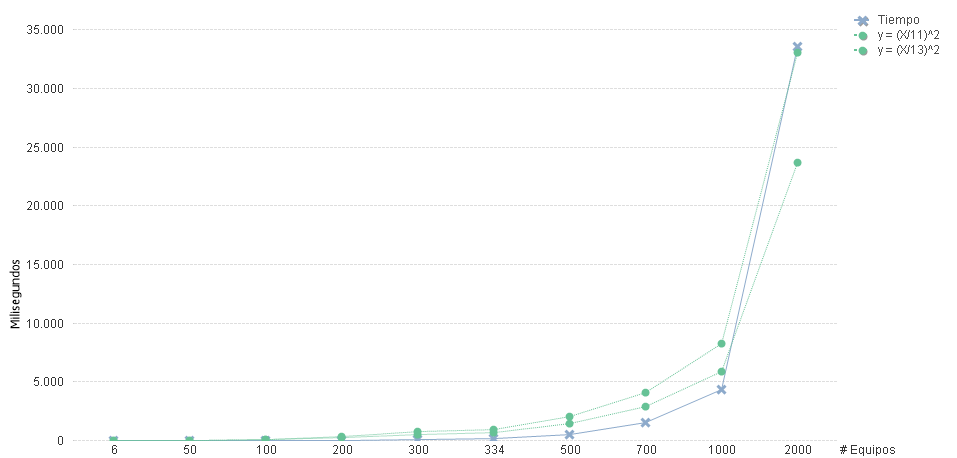
\includegraphics[width=1\textwidth]{IMG/gauss cuadrativo.png}
    \caption{Gauss cuadratico}
    \label{fig:Gauss cuadratico}
\end{figure}

\\

Luego observamos la misma gráfica pero con líneas de referencia de 2 funciones cubicas. \\

\begin{figure}[H]
    \centering
    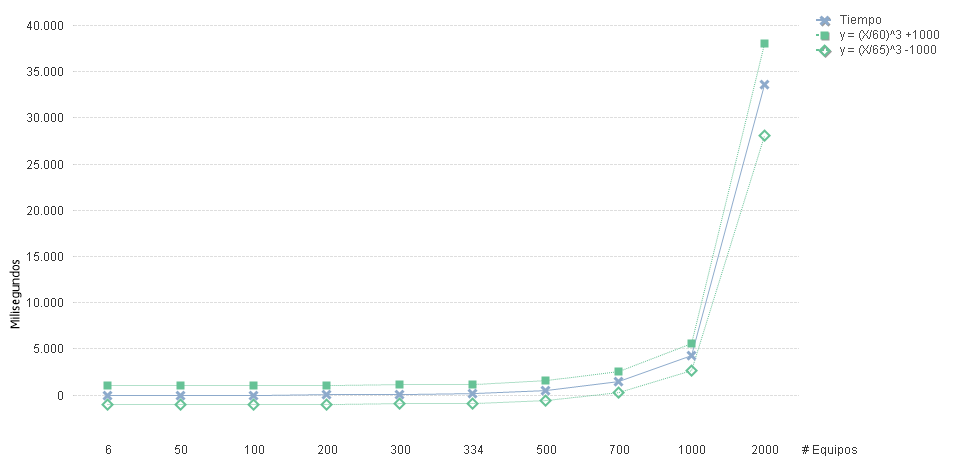
\includegraphics[width=1\textwidth]{IMG/gauss cubico.png}
    \caption{Gauss cubico}
    \label{fig:Gauss cubico}
\end{figure}

\\
Ejecutamos los test para nuestra implementación de Cholesky. A continuación se muestran los resultados de tiempos de ejecución dependiendo la cantidad de equipos.
Para mostrar la complejidad cúbica del algoritmo lo hemos encerrado entre 2 funciones cuadráticas que evidencian que no pueden contener la curva de tiempos de nuestro algoritmo.\\


\begin{figure}[H]
    \centering
    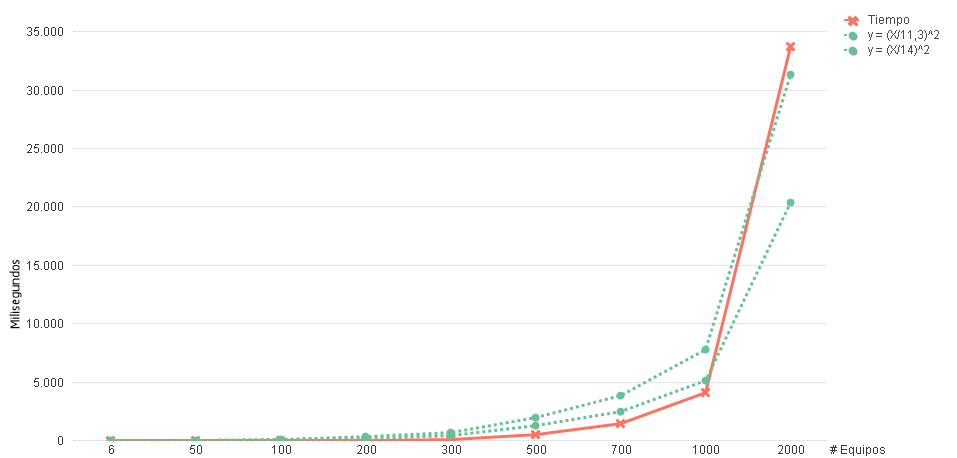
\includegraphics[width=1\textwidth]{IMG/cholesky cuadratico.png}
    \caption{Cholesky cuadratico}
    \label{fig:Cholesky cuadratico}
\end{figure}

\\

Luego observamos la misma grafica pero con líneas de referencia de 2 funciones cúbicas.\\

\begin{figure}[H]
    \centering
    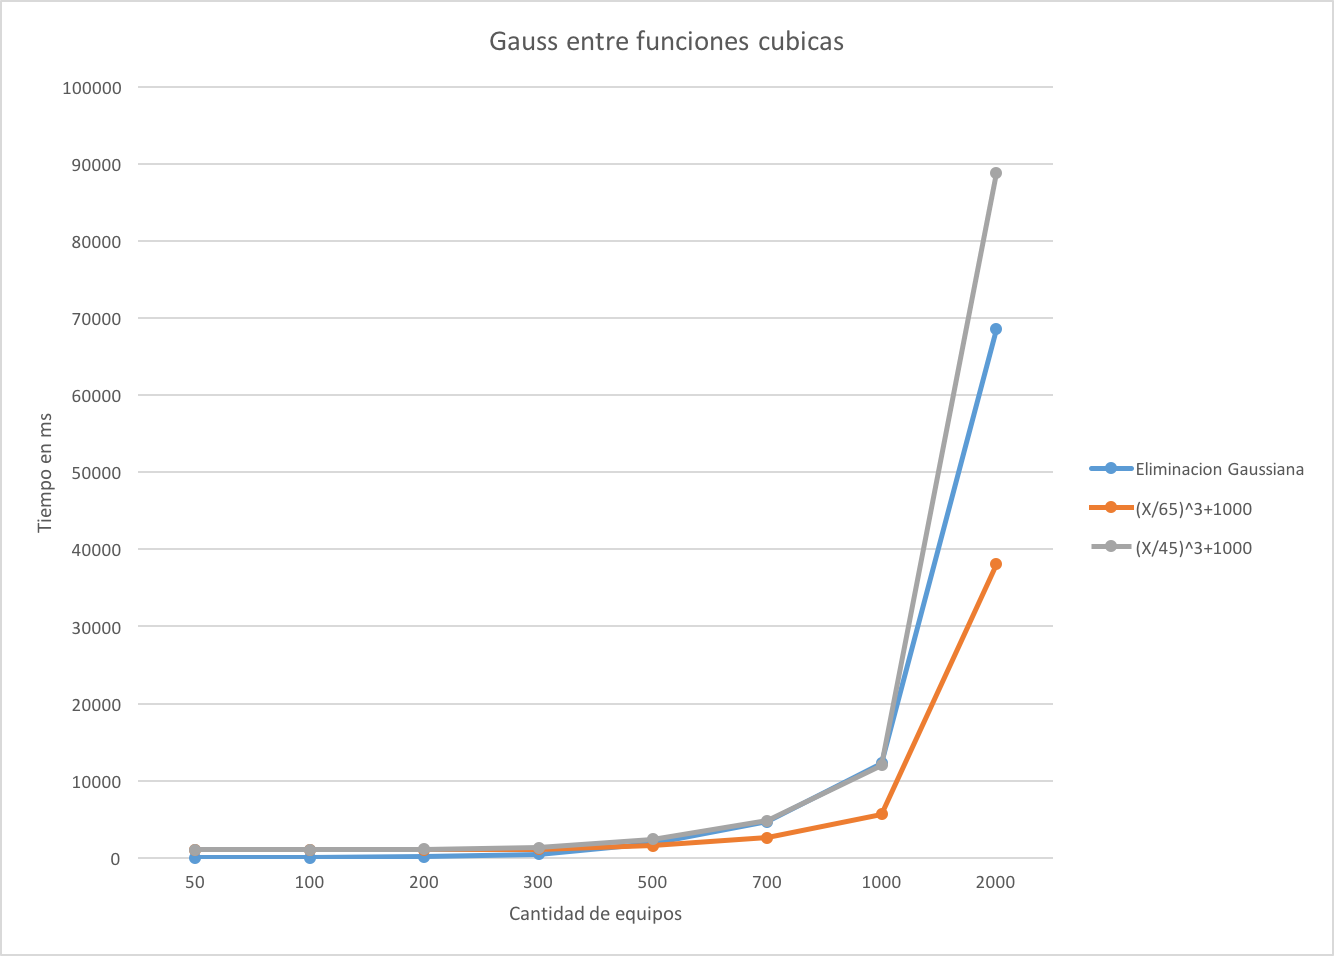
\includegraphics[width=1\textwidth]{IMG/gaussEntreCubicas.png}
    \caption{Cholesky cubico}
    \label{fig:Cholesky cubico}
\end{figure}

\\

Si comparamos ambos algoritmos, podemos comprobar que nuestra hipótesis de que Cholesky demora menos tiempo es correcta, como se puede ver en la siguiente gráfica.

\begin{figure}[H]
    \centering
    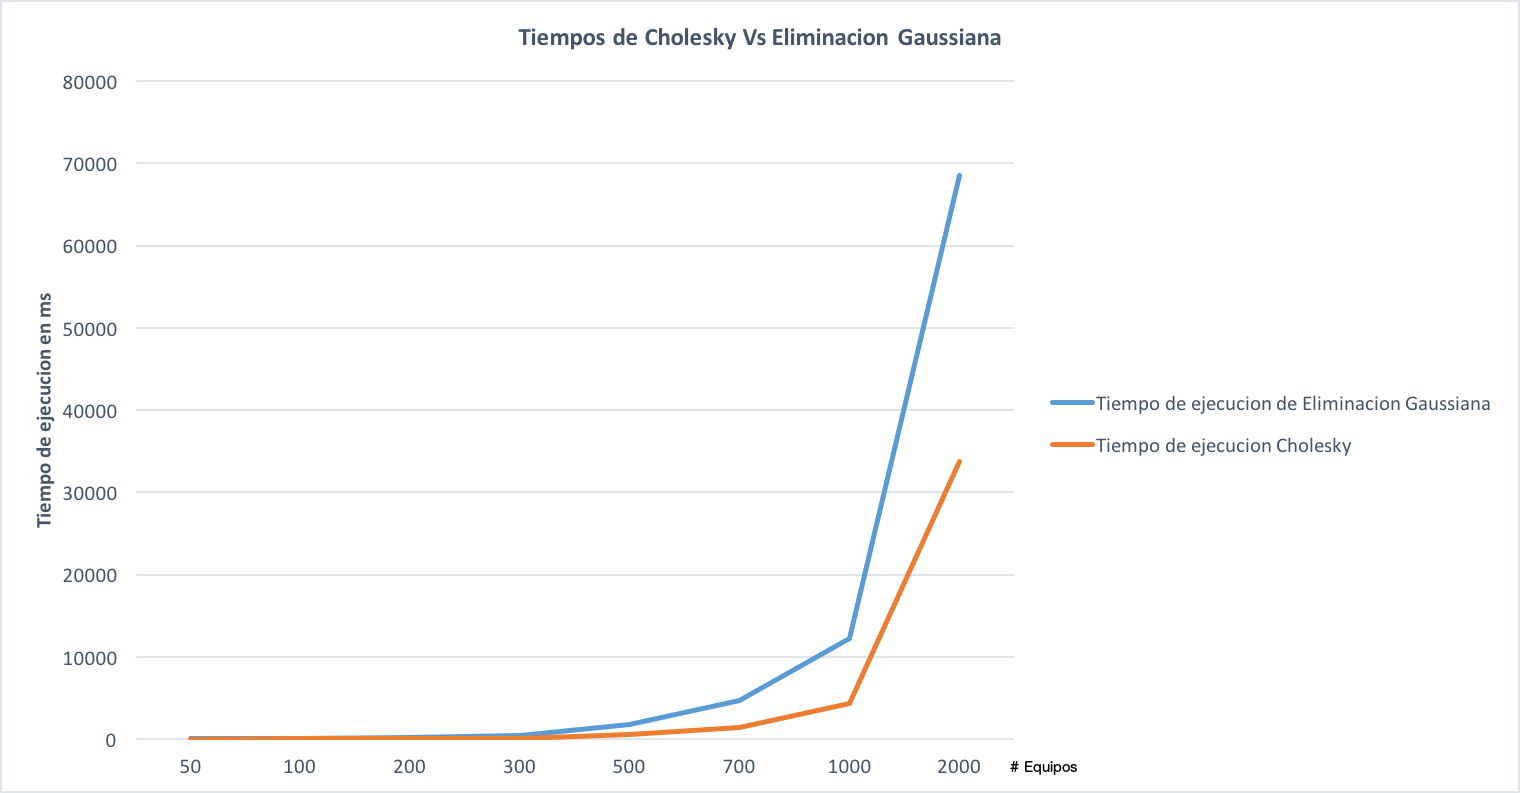
\includegraphics[width=1\textwidth]{IMG/tiemposgsvscholesky.png}
\end{figure}


Ejecutamos los test para nuestra implementación de WP. A continuación se muestran los resultados de tiempos de ejecución dependiendo la cantidad de equipos: \\


\begin{figure}[H]
    \centering
    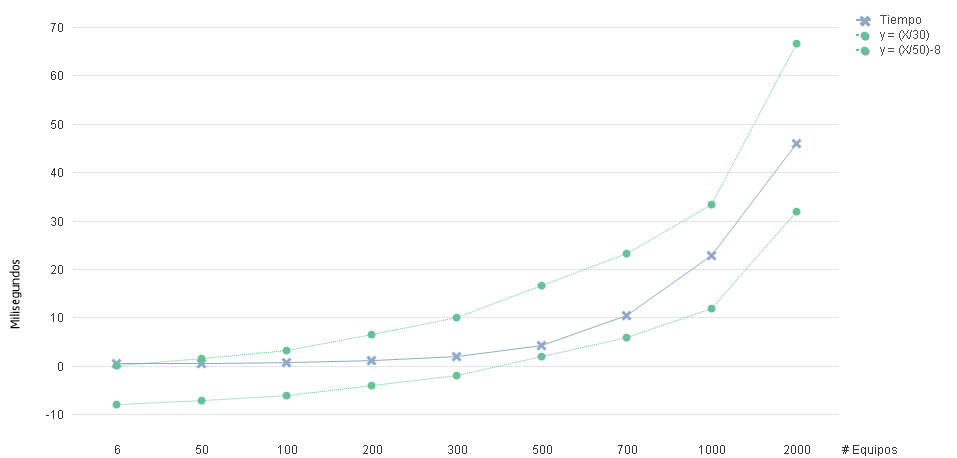
\includegraphics[width=1\textwidth]{IMG/wp lineal.png}
    \caption{WP lineal}
    \label{fig:WP lineal}
\end{figure}

\\
Cuando leímos el enunciado encontramos una frase que nos llamó la atención y era la siguiente: \\

Se pide comparar, para distintos tamaños de matrices, el tiempo de computo requerido para cada método en el contexto donde la información de la matriz del sistema $C$ se mantiene invariante,
pero varia el termino independiente $b$ \\

Como marcamos anteriormente, no hicimos uso de tener factorizada la matriz con el fin de acelerar los cálculos cuando modificamos el termino independiente, dado a que solamente hariamos uso del back substitution y forward substitution, ya que el cálculo de la factorización de Cholesky no requiere del termino independiente como si lo utiliza la eliminación gaussiana. Esto se puede apreciar mirando los algoritmos, donde Eliminación Gaussiana si hace uso del término independiente a diferencia de Cholesky que lo utiliza solo para los algoritmos de reemplazo. De haber realizado esto notaríamos cambios significativos en los tiempos de Cholesky para estas pruebas.
